\chapter{Documentation}

\section{Data Representation}

\section{Input data}

\section{Modules}
In this section, we describe the functionality of each program module. Third party software will not be described here. It can be found in \cref{chapt:technology}. Interactions between modules are described in \cref{fig:modules}. \emph{Irrlicht Engine} is not present in the diagram because we do not logically depend on using this engine. Every module is implemented in a file with the matching name as a class with the same name prefixed with letter M (Object Creator can be found in file ObjectCreator.cpp and is implemented as class {\tt gg::MObjectCreator}). Every component of this application is located in namespace {\tt gg};
\begin{description}
\item[Game]

\item[Event Receiver]
This class is an implementation of {\tt irr::IEventReceiver} from Irrlicht engine and it is used to read the user input.

\item[Loader]
The Loader is a class only used for initializing the application. It parses the data describing the game environment from the given file, constructs the objects with the help of {\tt gg::MObjectCreator} and returns the set of constructed objects.

\item[Object Creator]

\item[Collision Resolver]

\item[Mesh Manipulators]
Mesh Manipulators provides set of public static functions. Because different libraries are used for physics simulation, rendering and geometric manipulation, those functions provide means for converting data between different formats.
\end{description}

\begin{figure}
        \centering
        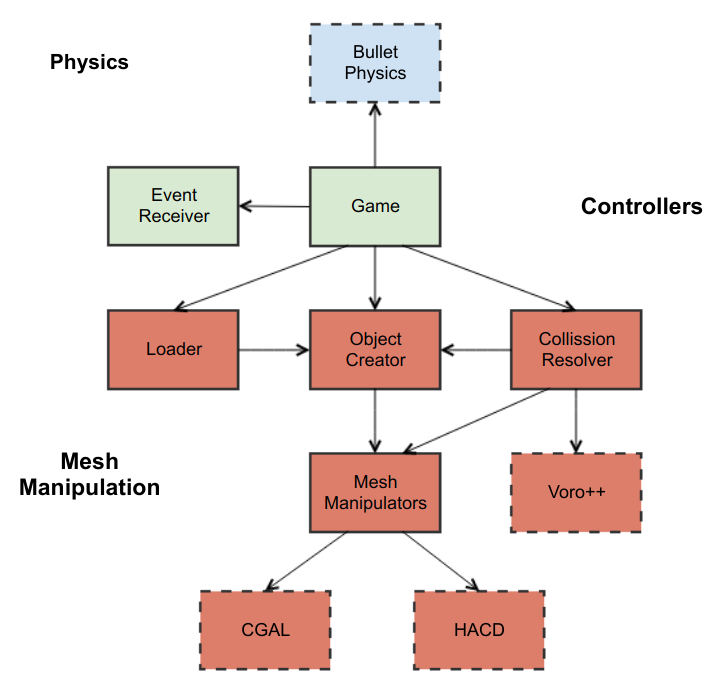
\includegraphics[width=\textwidth]{img/objectmodel}
        \caption{Software architecture shown on diagram of relationships of program modules. Third party software is highlighted in dashed rectangles.}
        \label{fig:modules}
\end{figure}

\section{Installation guide}

\section{User interface}
The user interface allows only for the use of the keyboard as follows:
\begin{itemize}
\item W/S: pitch down/up
\item A/D: roll counter-clockwise/clockwise 
\item Q/E: yaw left/right
\item Z/X: speed up/slow down
\item Space Bar: shoot or unpause
\item P: pause the game
\item ESC: quit the game
\end{itemize}
Keys can be pressed simultaneously and also held down instead of multiple presses.

